% =================================================================
%  IEEE Conference Paper
%  Title : Automated Multi-Domain Data Curation for
%          Cybersecurity-Focused Small Language Models
%
%  Overleaf Template (used as base):
%  https://www.overleaf.com/latex/templates/ieee-conference-template/grfzhhncsfqn
%
%  HOW TO USE ON OVERLEAF:
%  1. Open the link above and click "Open as Template"
%  2. Delete the default main.tex content
%  3. Paste or upload this entire file
%  4. Upload figures/dashboard_pipeline.jpg and figures/dashboard_dataset.jpeg
%     into a "figures" folder in the project
%  5. Click Compile
% =================================================================

\documentclass[conference]{IEEEtran}
\IEEEoverridecommandlockouts

% ---- Packages -----------------------------------------------
\usepackage{cite}
\usepackage{amsmath,amssymb,amsfonts}
\usepackage{graphicx}
\usepackage{textcomp}
\usepackage{xcolor}
\usepackage{url}
\usepackage{booktabs}
\usepackage{multirow}
\usepackage{array}
\usepackage{listings}
\usepackage{balance}

% ---- TikZ for flowcharts ------------------------------------
\usepackage{tikz}
\usetikzlibrary{shapes.geometric, arrows.meta, positioning, fit, backgrounds}

\tikzstyle{startstop} = [
    rectangle, rounded corners,
    minimum width=3.2cm, minimum height=0.7cm,
    text centered, draw=black, fill=blue!15,
    font=\small\bfseries]
\tikzstyle{process} = [
    rectangle,
    minimum width=3.2cm, minimum height=0.65cm,
    text centered, draw=black, fill=orange!15,
    font=\small]
\tikzstyle{subprocess} = [
    rectangle,
    minimum width=2.6cm, minimum height=0.6cm,
    text centered, draw=black, fill=orange!8,
    font=\scriptsize]
\tikzstyle{io} = [
    trapezium, trapezium left angle=75, trapezium right angle=105,
    minimum width=3.0cm, minimum height=0.65cm,
    text centered, draw=black, fill=green!15,
    font=\small]
\tikzstyle{decision} = [
    diamond, minimum width=2.8cm, minimum height=0.65cm,
    text centered, draw=black, fill=yellow!25, aspect=2.4,
    font=\scriptsize]
\tikzstyle{cloudbox} = [
    rectangle, rounded corners,
    minimum width=3.0cm, minimum height=0.6cm,
    text centered, draw=black, fill=purple!12,
    font=\scriptsize]
\tikzstyle{arrow} = [thick, ->, >=stealth]
\tikzstyle{dasharrow} = [thick, dashed, ->, >=stealth, gray]

% ---- Code listing style ------------------------------------
\lstset{
  basicstyle=\ttfamily\scriptsize,
  breaklines=true,
  frame=single,
  backgroundcolor=\color{gray!8},
  keywordstyle=\color{blue!70!black}\bfseries,
  commentstyle=\color{green!50!black},
  stringstyle=\color{red!60!black},
  numbers=left,
  numberstyle=\tiny\color{gray},
  numbersep=4pt
}

% =================================================================
\documentclass[conference]{IEEEtran}
% ...
\begin{document}
% ---- TITLE --------------------------------------------------
\title{CyberCorpus: An Automated Pipeline for\\
Multi-Domain Cybersecurity Data Collection}
% ---- AUTHORS ------------------------------------------------
\author{
  % ---- Row 1: symmetric blank + 2 authors + symmetric blank ----
  \IEEEauthorblockN{\ }
  \IEEEauthorblockA{\ }
  \and
  \IEEEauthorblockN{Yagnik Raval}
  \IEEEauthorblockA{
      \textit{Dept.\ of Information Technology}\\
      \textit{KJ Somaiya School of Engineering}\\
      Mumbai, India\\
      yagnik.raval@somaiya.edu}
  \and
  \IEEEauthorblockN{Vaibhav Shiroorkar}
  \IEEEauthorblockA{
      \textit{Dept.\ of Electronics and Computer Engineering}\\
      \textit{KJ Somaiya School of Engineering}\\
      Mumbai, India\\
      v.shiroorkar@somaiya.edu}
  \and
  \IEEEauthorblockN{\ }
  \IEEEauthorblockA{\ }
  % ---- Row 2: 3 authors ----
  \and
  \IEEEauthorblockN{Neil Sharma}
  \IEEEauthorblockA{
      \textit{Dept.\ of Electronics and Computer Engineering}\\
      \textit{KJ Somaiya School of Engineering}\\
      Mumbai, India\\
      neil.sharma@somaiya.edu}
  \and
  \IEEEauthorblockN{Vighnesh Dhotre}
  \IEEEauthorblockA{
      \textit{Dept.\ of Information Technology}\\
      \textit{KJ Somaiya School of Engineering}\\
      Mumbai, India\\
      vighnesh.dhotre@somaiya.edu}
  \and
  \IEEEauthorblockN{Dr. Ashwini Dalvi}
  \IEEEauthorblockA{
      \textit{Dept.\ of Information Technology}\\
      \textit{KJ Somaiya School of Engineering}\\
      Mumbai, India\\
      ashwinidalvi@somaiya.edu}
}
\maketitle
% ---- ABSTRACT -----------------------------------------------
\begin{abstract}
General-purpose large language models (LLMs) still underperform on
specialised security work. The limiting factor is usually the data, not
the size of the model: clean, licence-clear, domain-labelled
cybersecurity text is scarce and scattered across many sub-fields. We
present an automated curation pipeline that turns a heterogeneous,
allowlist-governed set of cybersecurity sources into a schema-validated,
training-ready dataset for a cybersecurity-focused Small Language Model
(SLM), covering twelve practice sub-domains plus a post-quantum
cryptography track. The pipeline fuses ingestion and cleaning into one
per-source worker and runs a five-step deterministic cleaning chain with
Presidio-based PII redaction. It enforces two independent admission
gates: a version-controlled allowlist that guards against source
substitution, and a default-deny licence classifier that keeps
encumbered content out of training. Surviving records pass two-tier
deduplication (exact hashing plus MinHash LSH at a Jaccard threshold of
0.65), a blocking sufficiency gate with drift tracking, and
normalisation onto a strict 22-field Pydantic v2 schema that keeps
collection-owned fields separate from placeholders reserved for
downstream labelling and annotation. The system runs on Prefect, DVC on
an S3 remote, and AWS ECS Fargate via Terraform, with a read-only
Streamlit dashboard and a tool-calling question-and-answer agent
grounded in the pipeline's own metadata. We report an active pilot over
192 catalogued sources, observed mid-run at 63 sources and 420
schema-valid records, in which the sufficiency gate correctly blocks
release when one source dominates a sub-domain. The pilot suggests that
a governance-first architecture, with independent admission gates, is a
practical and necessary basis for training data that stays trustworthy
and auditable for domain-adapted cybersecurity SLMs.
\end{abstract}

\begin{IEEEkeywords}
Cybersecurity, Small Language Models, Dataset Curation, Schema
Normalisation, MinHash LSH, Sufficiency Gating, Domain Adaptation,
Data Governance
\end{IEEEkeywords}

% =================================================================
\section{Introduction}

Cyber attacks keep growing in frequency, sophistication, and cost.
Global cybercrime is projected to reach \$12.2 trillion a year by 2031
\cite{braue2025cybercrime}. That pressure has driven strong demand for
automated security tooling, and natural language processing with LLMs
now sits at the centre of threat detection, vulnerability triage, and
incident response \cite{zhang2025llms}. Moving capable language models
into real security settings is harder than it looks, for two reasons
that bite hardest in this domain. The first is supply. Open,
high-quality, domain-specific pre-training material is scarce
\cite{yu2025primus}; cybersecurity text is fragmented and heterogeneous,
and much of it carries restrictive or unclear licensing. The second is
cost. Full-scale LLMs bring heavy compute and latency costs, and those
sit awkwardly with the on-premises and air-gapped environments common in
security operations \cite{levi2025cyberpal}.

Small Language Models (SLMs), broadly transformer models with fewer
than roughly three billion parameters \cite{minaee2024llm}, are a
compelling option. They run on commodity hardware and need no cloud.
Continually pre-trained on curated domain text, an SLM can match or beat
far larger general models on narrow technical tasks, where specialised
vocabulary counts for more than raw scale \cite{bayer2024cysecbert,
ferrag2024revolutionising}. All of that rests on one thing: a training
set that is broad, clean, and representative. To our knowledge, no
publicly documented pipeline clears that bar while also treating
governance, licensing, and dataset trustworthiness as core engineering
concerns rather than an afterthought.

This paper presents an automated curation pipeline that closes that
gap. The system ingests, cleans, gates, and normalises text from a
dual-gated set of cybersecurity sources covering twelve practice
sub-domains plus a post-quantum cryptography track, and outputs a
schema-validated, training-ready dataset for SLM pre-training. A plain
scrape-and-store design would treat collection as a single linear pass.
Ours instead treats every stage as a security boundary: a
version-controlled allowlist keeps a compromised upstream from entering
under a trusted name; a default-deny licence classifier independently
confirms the pipeline is entitled to train on a source; a blocking
sufficiency gate stops an under-represented sub-domain from reaching
release; and each release ships with a content-hashed provenance
manifest that makes a bad batch traceable and reversible.

\textbf{Contributions.} This paper contributes: (1)~a
governance-first, five-stage architecture (optional sourcing, fused
ingestion-and-cleaning, deduplication, a sufficiency gate, and
normalisation) in which no stage trusts its own input; (2)~a dual-gate
admission design that separates \emph{trust} (a version-controlled
allowlist against source substitution) from \emph{legality} (a
default-deny commercial-licence gate); (3)~a fused, per-source
ingestion-and-cleaning worker that deletes raw files immediately after
cleaning, bounding disk use without sacrificing parallelism; (4)~a
two-tier deduplication and blocking sufficiency-gate mechanism that
holds dataset integrity at scale with minimal oversight; (5)~a 22-field
canonical schema that separates collection-owned fields from explicit
placeholders for downstream labelling and annotation; and (6)~an
orchestration and deployment design on Prefect, DVC, and AWS ECS
Fargate, with a read-only dashboard and tool-calling Q\&A agent, plus an
empirical account of an active pilot including a worked example of the
sufficiency gate blocking release.

The rest of the paper reviews related work (Section~II), sets out the
methodology (Section~III) and its stage-by-stage implementation
(Section~IV), reports pilot results (Section~V), and concludes with
future work (Sections~VI--VII). The pipeline is implemented in Python
and is publicly available.\footnote{\url{https://github.com/vaibhavshiroorkar/cybersec-slm-data-collection}}

% =================================================================
\section{Related Work}

We survey work from 2022 to 2025 across four themes: LLMs and SLMs in
cybersecurity, domain-specific pre-training data, structured
threat-intelligence frameworks, and validation and privacy tooling.
Below, we focus on the works this design builds on or departs from.

\textbf{Models and domain data.} Zhang et al.\ \cite{zhang2025llms}
review LLMs across cybersecurity and single out hallucination and
missing domain knowledge as the dominant failure modes, pointing at
better data rather than prompting. Levi et al.\ \cite{levi2025cyberpal}
introduce CyberPal 2.0, a family of cybersecurity-expert SLMs and the
closest analogue to the model our dataset is meant to feed, while
SecureBERT \cite{aghaei2022securebert} and CySecBERT
\cite{bayer2024cysecbert} show that even modest domain adaptation
sharply improves security tasks, with Bayer et al.\ demonstrating that
quality beats volume. On collection, Yu et al.\ \cite{yu2025primus}
release Primus (a 15.9\% aggregate benchmark gain), and Penedo et al.\
\cite{penedo2023refinedweb} describe RefinedWeb, whose URL filtering,
language detection, and MinHash LSH cut a five-trillion-token crawl to
600 billion high-quality tokens. RefinedWeb is strictly linear, a
design we depart from by inserting a blocking sufficiency gate before
release. Lee et al.\ \cite{lee2022deduplication} show near-duplicate
removal both cuts memorisation and improves accuracy, and Abbas et al.\
\cite{abbas2023semdedup} propose semantic deduplication, which we note
as future work but replace with tractable lexical MinHash LSH here.

\textbf{Structured intelligence and infrastructure.} Al-Sada et al.\
\cite{alsada2025attck}, Rani et al.\ \cite{rani2024ttpxhunter}, and
Abdeen et al.\ \cite{abdeen2023smet} show that models aligned to MITRE
ATT\&CK and consistent, machine-readable provenance markedly outperform
zero-shot baselines at TTP extraction and CVE mapping, motivating a
resolved sub-domain on every record; Park and You
\cite{park2023pretrained} add that source-type diversity aids
generalisation, informing our multi-adapter ingestion. On tooling,
Leskovec et al.\ \cite{leskovec2014mmd} give the MinHash/LSH foundation,
Wang et al.\ \cite{wang2023selfinstruct} motivate splitting
collection-owned from annotation-owned fields, Pydantic v2
\cite{pydanticv2} makes strict closed-schema validation cheap, Presidio
\cite{presidio2023} backs PII redaction, Prefect \cite{prefect2023} and
DVC \cite{dvc2023} provide orchestration and versioning, and Schick et
al.\ \cite{schick2023toolformer} supply the tool-calling paradigm
behind our monitoring agent. Tihanyi et al.\ \cite{tihanyi2024cybermetric}
and Alam et al.\ \cite{alam2024ctibench} provide benchmarks for
evaluating the resulting SLM.


% =================================================================
\section{Methodology}

This section sets out the research design and the reasoning behind each
stage: why it is shaped as it is, what we rejected, and what justifies
the choice. Implementation is deferred to Section~IV, in the same order.

\subsection{Research Design}

We considered two ways to build a domain training set: filter an
existing general-web collection by keyword, or build a dedicated,
source-governed pipeline. We rejected the first: keyword-filtered
collections inherit the licensing and provenance gaps of the upstream
crawl, and cybersecurity text carries an outsized share of
research-only material \cite{yu2025primus}, so a post-hoc filter cannot
recover a clean licence trail. We adopted the second, a constructive
systems-research design \cite{penedo2023refinedweb} in which the
artefact is the pipeline and the contribution lies in the architectural
choices that make it general and deployable. Within that, we chose a
gated flow over a strictly linear one: a linear flow cannot stop an
under-represented sub-domain from silently reaching the training set,
whereas a blocking sufficiency check between cleaning and normalisation
can halt the run and force a return to ingestion. This matters most for
a young sub-field such as post-quantum cryptography, where permissively
licensed material is inherently thin. Three research questions guide the
design:

\textbf{RQ1.} How can an automated pipeline ingest cybersecurity
content from heterogeneous source types, dataset platforms,
scrapeable documents, crawlable sites, and structured feeds, while
preserving provenance, quality, and licence compliance under
independent governance controls?

\textbf{RQ2.} Which cleaning, redaction, and deduplication strategies
best produce a trustworthy, low-redundancy training set with minimal
manual intervention?

\textbf{RQ3.} Does a sufficiency-gated, schema-validated process yield
measurably more reliable data, by retention, sub-domain balance, and
duplicate-rejection rate, than an ungated linear pipeline?

\subsection{Source Governance and Domain Taxonomy}

Source governance is the pipeline's primary security boundary, and the
design reflects that. Every source is first classified against a fixed
taxonomy of twelve sub-domains: application, cloud, cryptography, data
privacy, governance and compliance, identity and access management
(IAM), incident response, malware analysis, network, penetration
testing, security operations, and threat intelligence. A parallel
post-quantum track shares the cryptography sub-domain but carries a
distinct domain code, so quantum-era material can be tracked separately
as the field matures.

Two independent gates then decide whether a classified source may be
fetched. We keep them separate because they answer different questions.
The \emph{allowlist} gate asks whether this exact source has been vetted
and trusted: sources under CC0-1.0, CC BY 4.0, Apache-2.0, or equivalent
public-domain terms are approved (they permit unrestricted downstream
use, including commercial deployment), while CC BY-SA, CC BY-NC,
GPL/AGPL, or unknown licences are rejected. The decision is recorded
once in a version-controlled allowlist, not re-derived at fetch time.
That guards against source substitution: a later-compromised or swapped
upstream cannot contribute under a trusted name unless its entry is
re-reviewed and re-committed. The \emph{commercial-licence} gate is
independent, and it asks a narrower legal question. Given a source's
recorded licence text, is the pipeline entitled to train commercially on
it? The catalogue's licence field is free text, spanning SPDX
identifiers, plain English, and named terms, so this gate is a
conservative, default-deny keyword classifier: anything not positively
recognised as unencumbered commercial text is blocked until a human
resolves the ambiguity. The separation earns its keep here. A source can
be a trusted catalogue member and still be blocked at fetch time when
its licence text is unfavourable, a distinction a single merged gate
could not express cleanly.

\subsection{Ingestion and Parallel Execution}

Ingestion is built around one idea: fuse ingestion and cleaning into a
single per-source unit of work instead of two sequential batch stages.
Running them sequentially would force every source's raw output to sit
on disk before cleaning could start, which does not scale to
multi-gigabyte sources. Fusing them lets each source's raw data be
deleted the moment it is cleaned, which caps peak disk use at roughly
one source's worth of raw data no matter how many sources run overall.

Sources also differ in access pattern: some are pulled through a
platform client library, some arrive as PDF or JSON documents, some
need an HTML parser or a headless browser, and structured feeds are
best consumed through a dedicated API. Rather than special-case this in
the orchestrator, we use one adapter per access pattern behind a
uniform fetch-and-normalise interface, so a new pattern is a new
adapter with no change to the parallel logic. Every crawlable-site
adapter also honours the target's \texttt{robots.txt}, so ingestion
respects publisher crawl policy as well as licence text. Because a
multi-hour run meets transient failures, rate limits, and crashes, each
source runs in its own worker process, and a per-source completion
ledger lets an interrupted run resume without re-fetching finished
sources.

\subsection{Cleaning and Quality Assurance}

Cleaning is a fixed, deterministic sequence of five steps rather than a
configurable filter chain, so the same raw record always yields the
same outcome. The order follows a dependency chain. Text is extracted
first into one prose field, so a feature-table row with no prose is
dropped here instead of being carried forward as noise. Anomalies are
then classified by severity: structural problems are dropped, while
behavioural anomalies a human might rescue are quarantined for review,
on the principle that an automated pipeline should default to
reversible actions. Deduplication comes early, since carrying a
duplicate through redaction and translation wastes work that is later
thrown away. PII redaction follows, before language handling, because
security text is unusually likely to carry incidental personal data
(analyst names, contact details in advisories, reporter emails) that
must not reach a training set. Language handling then translates and
keeps rather than filters and drops: removing a document purely for
being non-English discards usable signal, so only text that resists
translation, or that has no translation backend available, is dropped.
One rule holds across the whole stage: every step degrades to a
conservative, logged fallback instead of failing or silently changing
behaviour.

\subsection{Two-Tier Deduplication}

Deduplication runs in two tiers. The first uses exact content hashing
to reject byte-for-byte duplicates. It is nearly free relative to the
second tier, and it catches the common case of a source mirrored
verbatim across two platforms. The second uses MinHash LSH
\cite{leskovec2014mmd} for near-duplicates that are similar but not
identical, as with syndicated blog posts, mirrored advisories, and
forked repository docs. MinHash approximates the Jaccard similarity of
two documents represented as shingle sets $A$ and $B$:
\begin{equation}
  J(A, B) = \frac{|A \cap B|}{|A \cup B|}
\end{equation}
Using $k$ independent hash functions, the probability that the minimum
hash agrees for both sets equals $J(A,B)$. LSH then groups documents
into candidate pairs without an all-pairs comparison, which cuts
complexity from $O(n^2)$ to roughly $O(n)$ \cite{leskovec2014mmd}.

We set the Jaccard threshold to 0.65, lower than in many general-web
pipelines. The reason is boilerplate. Cybersecurity text is full of it:
CVE headers, advisory templates, repeated code. A looser threshold
catches template-level near-duplicates that a stricter one would miss,
at the acceptable cost of a slightly higher rejection rate. We also keep
a best-match score for every checked record, so the threshold can be
retuned against logged scores without re-running the comparison. One
more constraint shapes the design: a single global pass is memory-bound
at scale. So per-source workers run with duplicate checking disabled,
and one deterministic cross-source pass runs after the pool drains, so
duplicates that overlap only \emph{between} sources are still caught.

\subsection{Sufficiency Gating}

Analysis is only useful if it can act on what it finds, so the
exploratory-analysis stage is an enforcement point and not just a
report. Per sub-domain, it computes schema completeness, volume, source
concentration (whether one source dominates), text-quality indicators,
duplicate rate, and drift against the previous run. Violations split
into two severities. A \emph{blocker} (too few total records, or one
source exceeding a concentration ceiling) halts the pipeline and forces
a return to ingestion for that sub-domain, because such conditions make
a release structurally unreliable no matter how clean the text looks.
A \emph{warning} (a thin sub-domain, an elevated duplicate rate, low
average token length, or drift) is logged and tracked but does not stop
release, since it informs the next cycle without being disqualifying.
This blocker-versus-warning split is the main departure from a linear
pipeline such as RefinedWeb \cite{penedo2023refinedweb}: it lets the
pipeline guarantee a quality floor on every release instead of
reporting quality after the fact. Section~V shows the gate firing
during the pilot.

\subsection{Canonical Schema and Annotation Handoff}

The schema is built around one principle: every field is owned by
exactly one stage, or by a downstream team that has not run yet. Fields
the pipeline can compute with certainty (provenance, content hashes,
token and character counts, resolved domain and sub-domain) are filled
deterministically. Fields that depend on a weak-supervision labelling
pass or on human annotation get explicit typed placeholders instead of
being left absent, so the record shape is fixed and machine-readable
from the moment it is written. This buys two things. First, it stops an
annotation field from being silently overwritten by a later
re-ingestion, because collection-owned and annotation-owned fields are
structurally distinct. Second, it gives the labelling and annotation
teams a fixed contract, which supports the tooling-driven annotation of
Wang et al.\ \cite{wang2023selfinstruct} without the pipeline needing to
know their internals. We enforce the schema with Pydantic v2
\cite{pydanticv2} rather than a lighter option such as
\texttt{jsonschema}: its Rust core keeps enforcement cheap even with
all twenty-two fields validated per record, and \texttt{extra="forbid"}
rejects any unexpected field, so mapping bugs surface immediately
instead of letting malformed records drift downstream.

\subsection{Monitoring and Conversational Access}

A pipeline that gates its own release is only auditable if its state is
easy to inspect, so monitoring is a design requirement. The dashboard is
read-only. Pipeline state and dataset content share one surface, and the
dashboard only ever reads it: it never triggers a run, retries a source,
or edits a record, so exposing it more widely does not widen the attack
surface. On top of the same read layer we add a tool-calling agent. A
dashboard answers only the questions its designer anticipated, and a
free-text question, ``which sub-domain is thinnest right now?'', often
does not map onto a fixed page. Following the tool-calling paradigm
\cite{schick2023toolformer}, the agent gets a small fixed set of
read-only tools over the same data, and a model decides at inference
time which, if any, to invoke. No tool can write, retry, or reconfigure
anything, so the agent adds a natural-language interface to existing
observability without a new class of risk.

\subsection{System Architecture}

Fig.~\ref{fig:methodology_arch} shows the resulting architecture. An
optional sourcing stage proposes candidates for human review; nothing
it produces is trusted automatically. Ingestion applies both gates
before a source is fetched, and ingestion and cleaning run fused, per
source, in parallel, then hand off to a single cross-source
deduplication pass. The sufficiency gate then either releases the pooled data to
normalisation or forces a return to ingestion. Only after
normalisation, schema validation, and near-duplicate rejection does a
record reach the released dataset and its provenance manifest, which
feed the dashboard and its agent.

\begin{figure}[t]
\centering
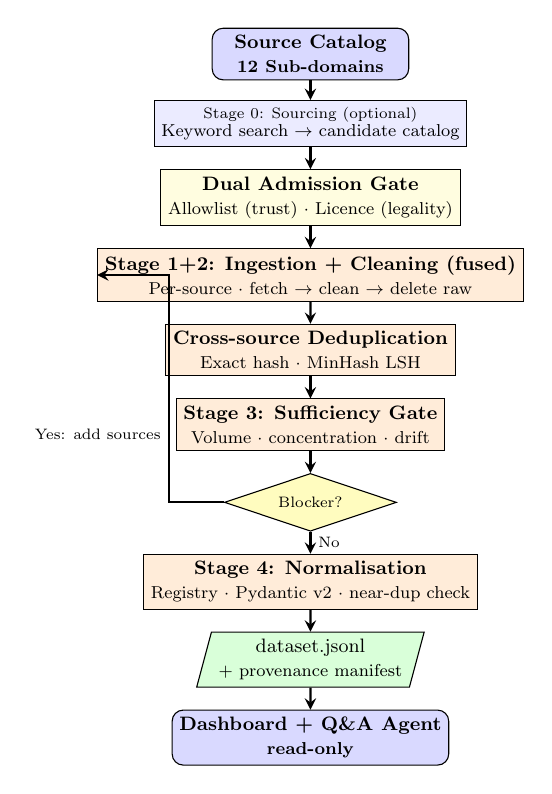
\begin{tikzpicture}[scale=0.78, transform shape, node distance=0.42cm, every node/.style={align=center}]

  \node (manifest) [startstop]
      {Source Catalog\\{\footnotesize 12 Sub-domains}};
  \node (s0) [subprocess, below=0.32cm of manifest, fill=blue!8]
      {Stage 0: Sourcing (optional)\\
       {\footnotesize Keyword search $\rightarrow$ candidate catalog}};
  \node (gates) [process, below=0.36cm of s0, fill=yellow!12]
      {\textbf{Dual Admission Gate}\\
       {\footnotesize Allowlist (trust) $\cdot$ Licence (legality)}};
  \node (s1) [process, below=0.36cm of gates]
      {\textbf{Stage 1+2: Ingestion + Cleaning (fused)}\\
       {\footnotesize Per-source $\cdot$ fetch $\rightarrow$ clean $\rightarrow$ delete raw}};
  \node (dedup) [process, below=0.36cm of s1]
      {\textbf{Cross-source Deduplication}\\
       {\footnotesize Exact hash $\cdot$ MinHash LSH}};
  \node (s3) [process, below=0.36cm of dedup]
      {\textbf{Stage 3: Sufficiency Gate}\\
       {\footnotesize Volume $\cdot$ concentration $\cdot$ drift}};
  \node (dec) [decision, below=0.36cm of s3]
      {Blocker?};
  \node (s4) [process, below=0.36cm of dec]
      {\textbf{Stage 4: Normalisation}\\
       {\footnotesize Registry $\cdot$ Pydantic v2 $\cdot$ near-dup check}};
  \node (s5) [io, below=0.36cm of s4]
      {dataset.jsonl\\{\footnotesize + provenance manifest}};
  \node (dash) [startstop, below=0.36cm of s5]
      {Dashboard + Q\&A Agent\\{\footnotesize read-only}};

  \draw [arrow] (manifest) -- (s0);
  \draw [arrow] (s0) -- (gates);
  \draw [arrow] (gates) -- (s1);
  \draw [arrow] (s1) -- (dedup);
  \draw [arrow] (dedup) -- (s3);
  \draw [arrow] (s3) -- (dec);
  \draw [arrow] (dec) -- node[right, font=\scriptsize] {No} (s4);
  \draw [arrow] (s4) -- (s5);
  \draw [arrow] (s5) -- (dash);
  \draw [arrow] (dec.west) -- ++(-0.9,0)
      |- node[left, font=\scriptsize, pos=0.15] {Yes: add sources} (s1.west);

\end{tikzpicture}
\caption{Conceptual pipeline architecture. Ingestion and cleaning run
fused, per source, in parallel, behind an independent allowlist and
licence check; a blocking sufficiency gate closes a feedback loop to
ingestion when a sub-domain is under-represented.}
\label{fig:methodology_arch}
\end{figure}

% =================================================================
\section{Implementation}

This section describes how the methodology is realised, in the same
order as Section~III.

\subsection{Technology Stack}

The pipeline is a Python 3.13 package, \texttt{cybersec\_slm}, managed
with the \texttt{uv} package manager (chosen for deterministic lock-file
resolution) and driven by one CLI, \texttt{cybersec-slm}. It follows a
stage-per-package layout with a per-stage \texttt{pytest} suite and
Terraform code alongside the source catalogue and allowlist. All
credentials are read from a \texttt{.env} file, never hard-coded, and
the whole run is invoked with \texttt{uv run cybersec-slm all}
(\texttt{--resume} skips finished sources); generated artefacts are
git-ignored, so the repository stays code-only.

\subsection{Source Governance}

The optional sourcing stage runs keyword searches per sub-domain, drops
already-catalogued URLs, and appends survivors in \texttt{pending}
status; nothing here reaches ingestion directly. The allowlist gate is a
version-controlled \texttt{allowlist.yaml} in which only
\texttt{approved} entries are fetched; it fails open only when the file
is absent, and an enforce flag (default in the Docker image) removes
even that. The independent commercial-licence gate then classifies the
lowercased, whitespace-collapsed licence string with a default-deny
keyword match, testing deny patterns before allow patterns so a compound
string such as ``CC BY-NC-SA 4.0'' is correctly blocked. The two gates
log with distinct reasons, so each stays independently auditable.

\subsection{Ingestion and Cleaning}

One worker handles one source end to end: it checks both gates, fetches
through the appropriate adapter, cleans in place, and deletes the raw
file before the next source is scheduled. Four adapters cover the main
access patterns: \textbf{fetch} for dataset-platform and repository sources
(HuggingFace, Kaggle, GitHub, raw URLs) via client libraries or HTTPX
with Tenacity retry; \textbf{scrape} for PDFs (PyMuPDF, preserving
page-level provenance) and JSON feeds; \textbf{html} for
robots.txt-permitted sites via \texttt{selectolax}, with headless
Playwright only for JavaScript-heavy pages; and \textbf{nvd} for the NVD
CVE REST API. A bad source returns \texttt{status="failed"} rather than
raising, so one malformed source cannot crash the pool; every outcome is
recorded in a SQLite log and a provenance ledger, and \texttt{--resume}
skips completed sources so an interrupted run never re-downloads a large
source. Cleaning then runs in the same worker in five fixed steps: text
mapping into one \texttt{text} field (pandas/Polars, dropping prose-less
rows); anomaly classification routing structural failures to
\texttt{dropped/} and behavioural anomalies to \texttt{flagged/}; exact
plus intra-source MinHash deduplication; PII redaction with Presidio
\cite{presidio2023} and a regex fallback; and language handling that
translates non-English text where possible and drops only what resists
translation. Each step degrades to a standard-library fallback and logs
the backend it used.

\subsection{Deduplication, Sufficiency Gate, and Normalisation}

After the pool drains, one deterministic cross-source pass processes
cleaned files in sorted order, so the surviving record of any
near-duplicate pair is stable across re-runs, and it is checkpointed per
file for resumability. The EDA stage then computes, per sub-domain,
schema completeness, volume, source concentration, quality, duplicate
rate, and drift against the previous run; a blocker fires when volume
falls below the minimum or a source's share exceeds the concentration
ceiling, and a warning for elevated duplicates or drift. Any blocker
raises \texttt{SufficiencyError} and halts the run before
normalisation; a \texttt{--no-enforce} flag downgrades the gate to
report-only.

Normalisation then maps every surviving record onto the 22-field
\texttt{CanonicalRecord} schema (Pydantic v2, \texttt{extra="forbid"},
closed enumerations). A mapper registry dispatches a \texttt{ProseMapper}
or a \texttt{StructuredMapper} (which renders table rows into readable
key-value sentences); an unknown shape raises a first-sight alert.
Enrichment fills what the mapper cannot: a uuid4 \texttt{id}, sha256
\texttt{content\_hash}, auto-computed \texttt{lang}, \texttt{token\_count},
and \texttt{char\_count}, version and timestamp, resolved domain and
sub-domain, and explicit placeholders (\texttt{-1}/ABSTAIN for the two
label fields, \texttt{null} for the four annotation fields). Validation
sends malformed records to a metadata-only reject log, a near-duplicate
MinHash LSH check at Jaccard 0.65 writes rejects to
\texttt{duplicates.jsonl}, and survivors are appended to
\texttt{dataset.jsonl} one line at a time. Table~\ref{tab:schema}
summarises the field groups; a release \texttt{manifest.json} then
records counts by domain, source, licence, format, and language, the EDA
snapshot, the git commit, and a sha256 of the dataset file, so every
release has a verifiable fingerprint.

\begin{table}[t]
\caption{Canonical Record Schema (22 Fields)}
\label{tab:schema}
\centering
\renewcommand{\arraystretch}{1.05}
\begin{tabular}{@{}p{1.7cm}p{1.5cm}p{4.0cm}@{}}
\toprule
\textbf{Group} & \textbf{Fields} & \textbf{Filled by} \\
\midrule
Identity & id, content\_hash & normalise \\
Content & text & clean $\rightarrow$ normalise \\
Provenance & source, source\_url, license, origin\_format & ingest \\
Auto-computed & lang, token\_count, char\_count & normalise \\
Pipeline meta & pipeline\_\allowbreak version, collected\_at & normalise \\
Labels & source\_file, record\_type, domain\_name, subdomain\_name, domain\_label, subdomain\_label & normalise (last two are \texttt{-1} placeholders) \\
Annotation & safe\_unsafe, confidence, instruction, reviewed\_by & \texttt{null} placeholders \\
\bottomrule
\end{tabular}
\end{table}

\subsection{Monitoring, Orchestration, and Deployment}

The dashboard is a Streamlit application with a strict read/render
split. One disk/SQLite module exposes pure functions, so the logic layer
is unit-testable without a browser. Its pages surface the live run
strip, gate outcome, EDA trends, and manifest; the released records in
full 22-field detail; and a chat interface. The agent exposes seven
read-only tools over the same data, each with server-side clamped result
sizes, and an NVIDIA NIM client drives a tool-calling loop
\cite{schick2023toolformer} bounded by six iterations. Every call is
wrapped so failures surface as error values, and nothing is persisted.
The read-only guarantee therefore holds even for the one networked
component.

Two orchestration paths wrap the same stage functions: a Prefect
\texttt{build-corpus} flow runs the fused ingest-and-clean step as
mapped, retried, isolated tasks (its decorators degrade to no-ops when
Prefect is absent, keeping stages testable), and DVC versions each
release against a remote store. Deployment targets AWS via Docker and
Terraform (ECR, ECS, S3, IAM, Secrets Manager): the build runs on ECS
Fargate, one task per scheduled run, reading keys from Secrets Manager at
runtime, and CI runs \texttt{gitleaks} and \texttt{pip-audit} alongside
\texttt{ruff} before an image is built. Least privilege holds
throughout: the task role touches only the one data bucket and four
named secrets, and the image carries no credentials.


% =================================================================
\section{Results}

\subsection{Pilot Instantiation and Current Run State}

At the time of writing the pipeline is feature-complete across all five
stages, the dual admission gate, and the monitoring dashboard with its
Q\&A agent, and it is in active operational use. Instead of a
hypothetical finished release, we describe what the running system
currently shows: an in-progress run targeting 192 allowlist-catalogued
sources, observed at 63 of 192 completed. Fig.~\ref{fig:dashboard_pipeline}
shows the Pipeline page from this run. At this point the cleaned dataset
holds 420 records across 4 of the 12 sub-domains, including IAM and
Threat Intelligence. We present this partial state as it stands, without
extrapolating from it: the aim is to show that the architecture behaves
as designed, not to claim a production-scale dataset.

\begin{figure}[t]
\centering
\includegraphics[width=0.86\columnwidth]{figures/dashboard_pipeline.jpg}
\caption{Dashboard Pipeline page captured mid-run: 63 of 192 sources
completed, a live per-source ingest log, and the sufficiency gate
reporting one active blocker.}
\label{fig:dashboard_pipeline}
\end{figure}

\subsection{The Sufficiency Gate Blocking Release}

The pilot gives a direct example of the blocking gate working as
intended. At the captured state it reports FAIL with one blocker and no
warnings: source \texttt{nist-sp800-63b} accounts for 100.0\% of the IAM
sub-domain, against a configured concentration ceiling of 60\%. Because
this is a blocker, the pipeline halts before normalisation and reports
the run as needing more IAM sources, rather than releasing a sub-domain
that is, in practice, one document repeated across many records. The
gate also reports 420 total records, a 0.0\% duplicate rate, an average
of 239 tokens per record, and 0.0\% drift (expected for an early run
with no prior snapshot). This is exactly the intended behaviour: a
genuinely under-diversified sub-domain is caught and blocked before it
can reach the released dataset.

\subsection{Ingestion, Fault Tolerance, and Schema Fidelity}

The same run log substantiates two design claims. First, the allowlist
gate is shown rejecting a source in real time: a candidate Kaggle
source, \texttt{dnkumars/\allowbreak cybersecurity-\allowbreak intrusion-\allowbreak detection-\allowbreak dataset}, is
skipped with reason \texttt{allowlist not approved} while an adjacent,
approved source from the same platform proceeds. This confirms the gate
discriminates per source, not per platform. Second, per-source worker
isolation absorbs a real failure: a large HuggingFace source
(\texttt{ealvaradob/phishing-dataset}, whose largest shard alone holds
871{,}590 rows at 696.7~MB) throws an \texttt{OSError} while writing one
shard, logged as \texttt{skip unreadable shard}, and the worker
continues with the remaining shards instead of crashing the run.

Fig.~\ref{fig:dashboard_dataset} shows the Dataset explorer filtered to
\texttt{nist-sp800-63b}. Each row shows a populated \texttt{id},
\texttt{source}, \texttt{subdomain\_name} (correctly resolved to IAM),
\texttt{record\_type} (\texttt{doc}), \texttt{token\_count},
\texttt{lang} (\texttt{en}), and \texttt{text} field. This confirms that
the 22-field schema of Table~\ref{tab:schema} is populated correctly end
to end for a real, structurally complex source: a NIST Special
Publication split into many section-level records.

\begin{figure}[t]
\centering
\includegraphics[width=0.86\columnwidth]{figures/dashboard_dataset.jpeg}
\caption{Dashboard Dataset explorer, filtered to \texttt{nist-sp800-63b}:
populated \texttt{id}, \texttt{source}, \texttt{subdomain\_name},
\texttt{record\_type}, \texttt{token\_count}, \texttt{lang}, and
\texttt{text} fields for each record.}
\label{fig:dashboard_dataset}
\end{figure}

% =================================================================
\section{Conclusion}

We presented an automated, governance-first pipeline for building a
schema-validated, multi-domain cybersecurity dataset for pre-training
cybersecurity-focused SLMs. The central contribution is architectural.
Instead of treating collection as a one-off scraping exercise, the
pipeline treats every stage as a security boundary that assumes its own
input may be untrustworthy, and it turns that stance into concrete
controls: a dual admission gate that separates a version-controlled
allowlist (against a substituted upstream) from an independent
default-deny licence classifier (against training on encumbered
content); a blocking sufficiency gate that keeps an under-filled or
over-concentrated sub-domain out of any release; strict schema
validation with closed enumerations; and a content-hashed provenance
manifest that makes every release traceable and reversible.

Several choices set this apart from the prior work of Section~II.
Fusing ingestion and cleaning into one per-source worker bounds peak
disk use without giving up parallelism, which matters at lab scale. The
blocker-versus-warning sufficiency gate is a structural safeguard
largely absent from linear pipelines such as RefinedWeb
\cite{penedo2023refinedweb}, and the pilot shows it at work: it caught a
sub-domain in which one source held 100\% of the content before that
imbalance could reach normalisation. Two-tier deduplication, with a
threshold tuned for cybersecurity boilerplate, follows the value of
aggressive redundancy control \cite{lee2022deduplication} without an
infeasible all-pairs comparison. The orchestration layer shows that a
student-built pipeline can adopt production discipline, no-op-degrading
Prefect decorators, DVC-versioned releases, least-privilege IAM,
without losing the unit-testability a lab needs. These results come from
an active, in-progress run and not a finished release. They should be
read as evidence that the architecture behaves as designed, including
under a real gate-blocking condition, and not as a claim of a completed
dataset. The path to a larger release is mainly operational: finishing
the remaining 129 sources and clearing the current IAM concentration
blocker.

% =================================================================
\section{Future Work}

Several directions would extend this pipeline. The most immediate is to
finish the pilot: clear the IAM concentration blocker with additional
non-dominant sources and progress the catalogue until the gate passes
across all twelve sub-domains, at which point a full, manifest-backed
release with final retention and rejection statistics can be reported.
The schema already anticipates a weak-supervision labelling pass. A
snorkel-style label model over the placeholder label fields would
replace the ABSTAIN defaults without a schema change, and would pair
with active-learning-driven annotation that spends scarce annotator time
on the records the model is least sure about. Embedding-based semantic
deduplication \cite{abbas2023semdedup}, added as a hybrid pass over
records that survive lexical dedup, would catch paraphrased
near-duplicates that MinHash misses, common in mirrored CVE summaries.
Scheduled incremental ingestion against live feeds (the NVD CVE API,
the CISA Known Exploited Vulnerabilities catalogue, vendor advisories)
would keep the dataset current; it would reuse the existing resume
ledger for checkpointing and need only a change-detection layer.
Finally, two pieces of hardening remain. Extending PII redaction to
internal hostnames, private IP ranges, service-account identifiers, and
embedded credentials would close a documented blind spot that is
disproportionately common in security text; completing the operational
hardening already underway would take the pipeline from a validated,
in-progress architecture to a production-ready service that sustains a
living, continuously updated dataset.

% =================================================================
\begin{thebibliography}{00}
\scriptsize
\setlength{\itemsep}{0pt}
\setlength{\parskip}{0pt}

\bibitem{braue2025cybercrime}
D. Braue,
``Cybercrime to cost the world \$12.2 trillion annually by 2031,''
\textit{Cybersecurity Ventures}, 2025.
[Online]. Available: \url{https://cybersecurityventures.com}

\bibitem{zhang2025llms}
J. Zhang, H. Bu, H. Wen, Y. Liu, H. Fei, R. Xi, L. Li, Y. Yang,
H. Zhu, and D. Meng,
``When LLMs meet cybersecurity: A systematic literature review,''
\textit{Cybersecurity}, vol. 8, no. 1, pp. 1--41, 2025.

\bibitem{levi2025cyberpal}
M. Levi et al.,
``Toward cybersecurity-expert small language models,''
\textit{arXiv preprint arXiv:2510.14113}, 2025.

\bibitem{yu2025primus}
Y.-C. Yu, T.-H. Chiang, C.-W. Tsai, C.-M. Huang, and W.-K. Tsao,
``Primus: A pioneering collection of open-source datasets for
cybersecurity LLM training,''
in \textit{Proc. 2025 Conf. on Empirical Methods in Natural Language
Processing (EMNLP)},
Suzhou, China, pp. 10391--10413, 2025.

\bibitem{aghaei2022securebert}
E. Aghaei, X. Niu, W. Shadid, and E. Al-Shaer,
``SecureBERT: A domain-specific language model for cybersecurity,''
in \textit{Proc. 18th EAI Int. Conf. on Security and Privacy in
Communication Networks (SecureComm)},
Springer, 2022, pp. 39--56.

\bibitem{bayer2024cysecbert}
M. Bayer, P. Kuehn, R. Shanehsaz, and C. Reuter,
``CySecBERT: A domain-adapted language model for the cybersecurity
domain,''
\textit{ACM Trans. Privacy and Security}, vol. 27, no. 2,
pp. 1--20, 2024.

\bibitem{alsada2025attck}
B. Al-Sada, A. Sadighian, and G. Oligeri,
``MITRE ATT\&CK: State of the art and way forward,''
\textit{ACM Comput. Surv.}, vol. 57, no. 1, pp. 1--37, 2025.

\bibitem{rani2024ttpxhunter}
N. Rani, B. Saha, V. Maurya, and S. K. Shukla,
``TTPXHunter: Actionable threat intelligence extraction as TTPs
from finished cyber threat reports,''
\textit{Digital Threats: Research and Practice}, vol. 5, no. 4,
pp. 1--19, 2024.

\bibitem{ferrag2024revolutionising}
M. A. Ferrag, M. Ndhlovu, N. Tihanyi, L. C. Cordeiro, M. Debbah,
T. Lestable, and N. S. Thandi,
``Revolutionizing cyber threat detection with large language models:
A privacy-preserving BERT-based lightweight model for IoT/IIoT
devices,''
\textit{IEEE Access}, vol. 12, pp. 68280--68297, 2024.

\bibitem{park2023pretrained}
Y. Park and W. You,
``A pretrained language model for cyber threat intelligence,''
in \textit{Proc. 2023 Conf. on Empirical Methods in Natural Language
Processing: Industry Track},
Association for Computational Linguistics, 2023, pp. 113--122.

\bibitem{lee2022deduplication}
K. Lee, D. Ippolito, A. Nystrom, C. Zhang, D. Eck,
C. Callison-Burch, and N. Carlini,
``Deduplicating training data makes language models better,''
in \textit{Proc. 60th Annual Meeting of the ACL},
Dublin, Ireland, pp. 8424--8445, 2022.

\bibitem{penedo2023refinedweb}
G. Penedo, Q. Malartic, D. Hesslow, R. Cojocaru, H. Alobeidli,
A. Cappelli, B. Pannier, E. Almazrouei, and J. Launay,
``The RefinedWeb dataset for Falcon LLM: Outperforming curated
corpora with web data, and web data only,''
in \textit{Proc. 37th Conf. on Neural Information Processing Systems
(NeurIPS), Datasets and Benchmarks Track},
New Orleans, USA, 2023.

\bibitem{abbas2023semdedup}
A. Abbas, K. Tirumala, D. Simig, S. Ganguli, and A. S. Morcos,
``SemDeDup: Data-efficient learning at web-scale through semantic
deduplication,''
\textit{arXiv preprint arXiv:2303.09540}, 2023.

\bibitem{minaee2024llm}
S. Minaee, T. Mikolov, N. Nikzad, M. Chenaghlu, R. Socher,
X. Amatriain, and J. Gao,
``Large language models: A survey,''
\textit{arXiv preprint arXiv:2402.06196}, 2024.

\bibitem{leskovec2014mmd}
J. Leskovec, A. Rajaraman, and J. D. Ullman,
\textit{Mining of Massive Datasets}, 2nd ed.
Cambridge, UK: Cambridge University Press, 2014.

\bibitem{pydanticv2}
S. Colvin et al.,
``Pydantic v2: Data validation using Python type hints,''
\textit{Pydantic Documentation}, 2023.
[Online]. Available: \url{https://docs.pydantic.dev/latest/}

\bibitem{wang2023selfinstruct}
Y. Wang, Y. Kordi, S. Mishra, A. Liu, N. A. Smith, D. Khashabi,
and H. Hajishirzi,
``Self-instruct: Aligning language models with self-generated
instructions,''
in \textit{Proc. 61st Annual Meeting of the ACL},
Toronto, Canada, pp. 13484--13508, 2023.

\bibitem{abdeen2023smet}
B. Abdeen, E. Al-Shaer, A. Singhal, L. Khan, and K. Hamlen,
``SMET: Semantic mapping of CVE to ATT\&CK and its application
to cybersecurity,''
in \textit{IFIP Annual Conf. on Data and Applications Security
and Privacy},
Springer, 2023, pp. 243--260.

\bibitem{schick2023toolformer}
T. Schick, J. Dwivedi-Yu, R. Dess\`i, R. Raileanu, M. Lomeli,
L. Zettlemoyer, N. Cancedda, and T. Scialom,
``Toolformer: Language models can teach themselves to use tools,''
in \textit{Proc. 37th Conf. on Neural Information Processing Systems
(NeurIPS)},
New Orleans, USA, 2023.

\bibitem{tihanyi2024cybermetric}
N. Tihanyi, T. Bisztray, R. Jain, M. A. Ferrag, L. C. Cordeiro,
and V. Mavroeidis,
``CyberMetric: A benchmark dataset based on retrieval-augmented
generation for evaluating LLMs in cybersecurity knowledge,''
\textit{arXiv preprint arXiv:2402.07688}, 2024.

\bibitem{alam2024ctibench}
M. T. Alam, D. Bhusal, Y. Park, and N. Rastogi,
``CTIBench: A benchmark for evaluating LLMs in cyber threat
intelligence,''
\textit{arXiv preprint arXiv:2406.07599}, 2024.

\bibitem{presidio2023}
Microsoft,
``Presidio: Context aware, pluggable and customizable PII
de-identification service,''
\textit{Microsoft Open Source Documentation}, 2023.
[Online]. Available: \url{https://microsoft.github.io/presidio/}

\bibitem{prefect2023}
Prefect Technologies,
``Prefect: The easiest way to orchestrate and observe your data
pipelines,''
\textit{Prefect Documentation}, 2023.
[Online]. Available: \url{https://docs.prefect.io}

\bibitem{dvc2023}
Iterative.ai,
``DVC: Data version control for machine learning projects,''
\textit{DVC Documentation}, 2023.
[Online]. Available: \url{https://dvc.org}

\end{thebibliography}

\end{document}